% !TeX root = ../summary-syssec.tex

\section{IoT}
\subsection{Light bulbs go nuclear}
\begin{enumerate}
    \item extract firmware update signing key using differential power analysis
    \item circumvent proximity checks
    \item make bulb join malicious network
    \item perform OTA firmware update
\end{enumerate}
Note: classical defence mechanisms like firewalls are not effective

Works because firmware only includes a MAC and is not signed (asymmetrically), therefor extracted key can \textit{sign} new firmware updates.

\subsubsection{Encrypt everything?}
\textbf{Not sufficient}! device identifiers, traffic volume still leak information, activities

\begin{description}
    \item[existential leakage] single transmission implies real-world event
    \item[statistical leakage] deviation from normal implies real-world event
\end{description}

\subsubsection{Hide transmission times and encrypt?}
\textbf{Not sufficient}! Examples: 
\begin{itemize}
    \item VOIP word reconstruction from encrypted packages (leak from variable bit length encoding and length-preserving encryption).
    \item side-channel leaks of web apps by analysing traffic
\end{itemize}

\begin{center}
    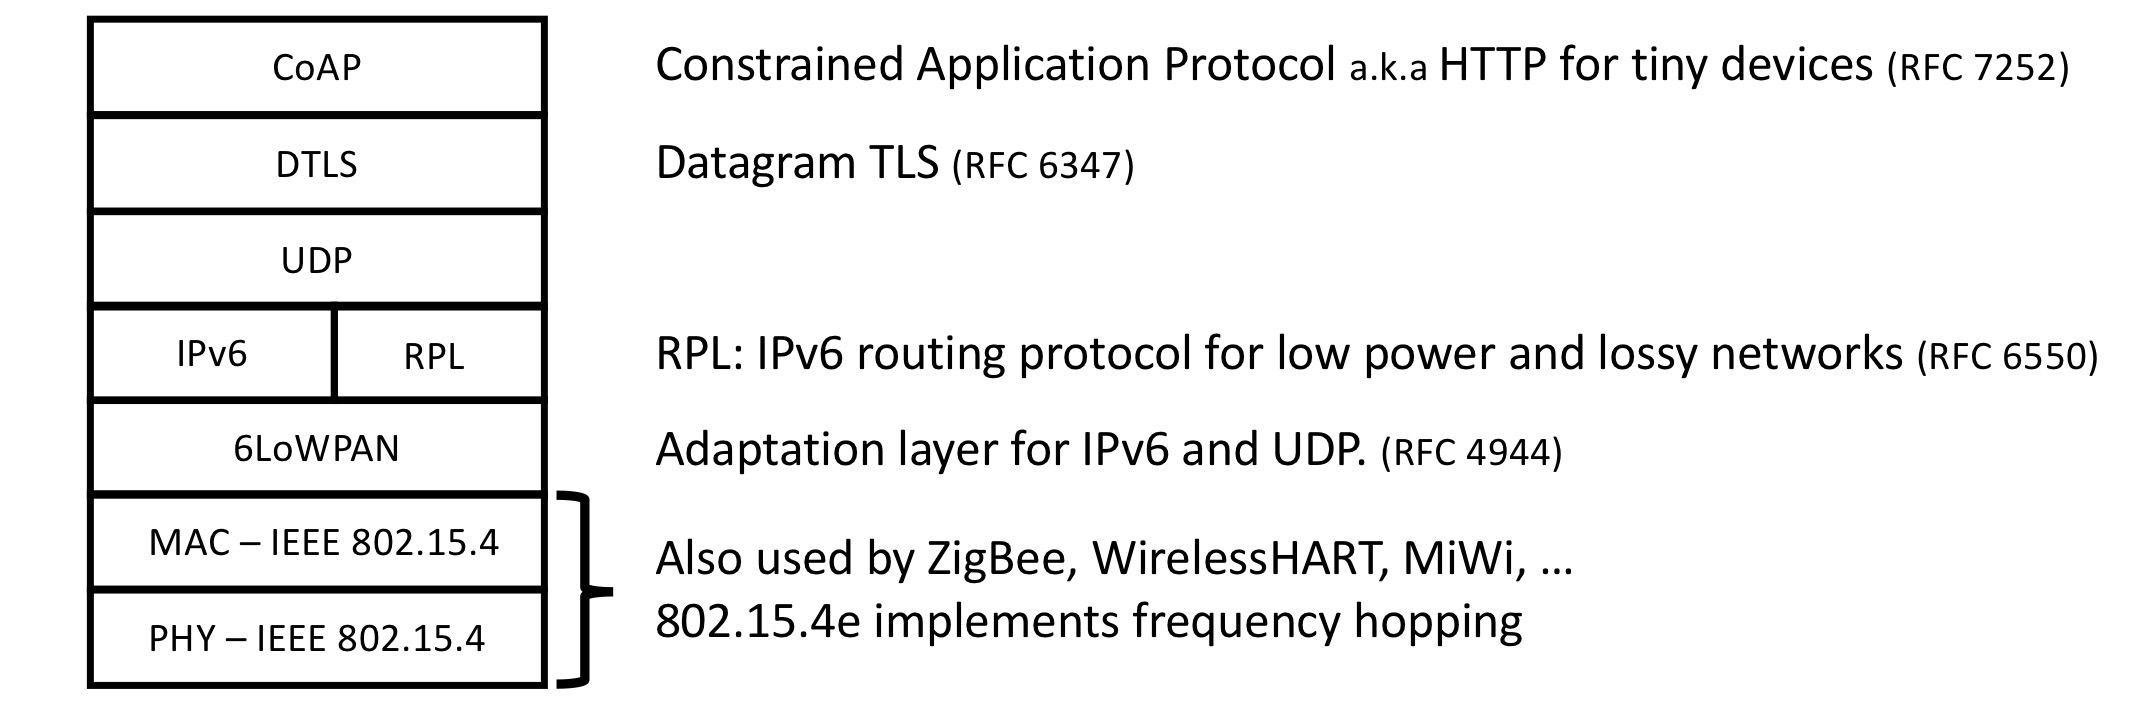
\includegraphics[width=\linewidth]{images/iot_stack}
\end{center}

\subsection{Device Pairing}
\begin{description}
    \item[Pairing] process of establishing a security association between two devices without prior shared knowledge
    \item[security association] can be anything only known to paired devices (e.g. secret key)
\end{description}

Paring method shall minimise I/O hardware needed and avoid complex user interactions.

\begin{description}
    \item[Out-of-band] extra channel which guarantees authenticity and is assumed to be secure even under MITM attack
    \item[In-band] often relies on physical channel properties and use special encoding (etc.) to detect MITM attack easily.
\end{description}